\documentclass[11pt]{article}

% some definitions for the title page
\newcommand{\reporttitle}{NLP and Classificaiton}
\newcommand{\reportdescription}{Intro to how one would develop classification algorithms for natural language processing}

% load some definitions and default packages
%---------------------------------------------------------------------------
%	PACKAGES AND OTHER DOCUMENT CONFIGURATIONS
%---------------------------------------------------------------------------

\usepackage[twoside]{fancyhdr}
\usepackage{csquotes}

\usepackage[a4paper,hmargin=2.0cm,vmargin=1.0cm,includeheadfoot]{geometry}
% \usepackage{natbib} % for bibliography
\usepackage{biblatex}
\usepackage{tabularx,longtable,multirow,subfigure,caption}%hangcaption
\usepackage{fancyhdr} % page layout
\usepackage{url} % URLs
\usepackage[english]{babel}
\usepackage{graphicx}
\usepackage{rotating}
\usepackage{dsfont}
\usepackage{epstopdf} % automatically replace .eps with .pdf in graphics
% \usepackage{backref} % needed for citations
\usepackage{array}
\usepackage{latexsym}
\usepackage[pdftex,hypertexnames=false,colorlinks]{hyperref} % provide links in pdf (had pagebackref)
\usepackage{booktabs}
\usepackage{wrapfig}
\usepackage{caption}  % Required for \captionof
\usepackage{float} % for H option in figures
\usepackage{amssymb}
\usepackage{amsmath}
\usepackage{amsthm}
\usepackage{mathtools} % for 'dcases*' env.
\usepackage[nottoc]{tocbibind}

%%% Default fonts
\renewcommand*{\rmdefault}{bch}
\renewcommand*{\ttdefault}{cmtt}

%%% Default settings (page layout)
\setlength{\parindent}{0em}  % indentation of paragraph
\setlength{\parskip}{.3em}
\setlength{\itemsep}{0.mm}

\setlength{\headheight}{14.5pt}
\pagestyle{fancy}

\fancyfoot[ER,OL]{\thepage}%Page no. in the left on odd pages and on right on even pages

\fancyfoot[OC,EC]{\sffamily }
\renewcommand{\headrulewidth}{0.1pt}
\renewcommand{\footrulewidth}{0.1pt}
\captionsetup{margin=10pt,font=small,labelfont=bf}

% LISTINGS ammendments
\usepackage{listings}
\usepackage{color}

\definecolor{mygreen}{rgb}{0,0.6,0}
\definecolor{mygray}{rgb}{0.5,0.5,0.5}
\definecolor{mymauve}{rgb}{0.58,0,0.82}

\lstset{ 
  postbreak=\mbox{\textcolor{red}{$\hookrightarrow$}\space},
  backgroundcolor=\color{white},   % choose the background color; you must add \usepackage{color} or \usepackage{xcolor}; should come as last argument
  basicstyle=\footnotesize,        % the size of the fonts that are used for the code
  breakatwhitespace=false,         % sets if automatic breaks should only happen at whitespace
  breaklines=true,                 % sets automatic line breaking
  captionpos=b,                    % sets the caption-position to bottom
  commentstyle=\color{mygreen},    % comment style
%   deletekeywords={...},            % if you want to delete keywords from the given language
%   escapeinside={\%*}{*)},          % if you want to add LaTeX within your code
  extendedchars=true,              % lets you use non-ASCII characters; for 8-bits encodings only, does not work with UTF-8
  firstnumber=1,                % start line enumeration with line 1000
  frame=single,	                   % adds a frame around the code
  keepspaces=true,                 % keeps spaces in text, useful for keeping indentation of code (possibly needs columns=flexible)
  columns=fullflexible,
  keywordstyle=\color{blue},       % keyword style
  language=python,                 % the language of the code
  % morekeywords={*,...},            % if you want to add more keywords to the set
  numbers=left,                    % where to put the line-numbers; possible values are (none, left, right)
  numbersep=5pt,                   % how far the line-numbers are from the code
  numberstyle=\tiny\color{mygray}, % the style that is used for the line-numbers
  rulecolor=\color{black},         % if not set, the frame-color may be changed on line-breaks within not-black text (e.g. comments (green here))
  showspaces=false,                % show spaces everywhere adding particular underscores; it overrides 'showstringspaces'
  showstringspaces=false,          % underline spaces within strings only
  showtabs=false,                  % show tabs within strings adding particular underscores
  stepnumber=1,                    % the step between two line-numbers. If it's 1, each line will be numbered
  stringstyle=\color{mymauve},     % string literal style
  tabsize=2,	                   % sets default tabsize to 2 spaces
  title=\lstname% show the filename of files included with \lstinputlisting; also try caption instead of title
}

% Here, you can define your own macros. Some examples are given below.

\newcommand{\R}[0]{\mathds{R}} % real numbers
\newcommand{\Z}[0]{\mathds{Z}} % integers
\newcommand{\N}[0]{\mathds{N}} % natural numbers
\newcommand{\C}[0]{\mathds{C}} % complex numbers
\renewcommand{\vec}[1]{{\boldsymbol{{#1}}}} % vector
\newcommand{\mat}[1]{{\boldsymbol{{#1}}}} % matrix


\bibliography{../bibliography}

\begin{document}

% Include the title page
\begin{titlepage}

    \newcommand{\HRule}{\rule{\linewidth}{0.5mm}} % Defines a new command for the horizontal lines, change thickness here
    
    \center % Center everything on the page
     
    %------------------------------------------------------------------------
    %	HEADING SECTIONS
    %------------------------------------------------------------------------
    
    \textsc{\Large Department of Computing}\\[0.5cm] 
    \textsc{\large Imperial College of Science, Technology and Medicine}\\[0.5cm] 
    
    %------------------------------------------------------------------------
    %	TITLE SECTION
    %------------------------------------------------------------------------
    
    \HRule \\[0.4cm]
    { \huge \bfseries \reporttitle}\\ % Title of your document
    \HRule \\[0.4cm]

    \textit{\reportdescription}
    
    \vspace{2em}

    %------------------------------------------------------------------------
    %	AUTHOR SECTION
    %------------------------------------------------------------------------
    
    \large \emph{Author: Anton Zhitomirskiy}

    \vspace{1em}

    \global\let\newpagegood\newpage
    \global\let\newpage\relax
    
\end{titlepage}

\global\let\newpage\newpagegood

\tableofcontents

\clearpage

\section{Classification}

\subsection{NLP Classification tasks}

\begin{definition}[Classification]
    \begin{equation}
        \hat{y} = \arg\max_y P(y|x)    
    \end{equation}
    Predicting which `class' an observation belongs to
\end{definition}

A Model produces a score (logit), a sigmoid makes this between 0 and 1, and 0.5 is our decision boundary. In multi-class classification we then use softmax.

\subsubsection{Natural Language Inference}

a model is presented with a pair of sentences and must classify the relationship between their meanings. For example in the MultiNLI corpus, pairs of sentences are given one of 3 labels: entails, contradicts and neutral. These labels describe a relationship between the meaning of the first sentence (the premise) and the meaning of the second sentence (the hypothesis)~\cite{book-speech-and-language-processing}. Here are representative examples of each class from the corpus:

\begin{itemize}
    \item \textbf{Premise}: The kitten is climbing the curtains again
    \item \textbf{Hypothesis}: The kitten is sleeping
    \item \textbf{Entailment}: If the hypothesis is implied by the premise
    \item \textbf{Contradiction}: If the hypothesis contradicts the premise (in this example, the hypothesis is contradicting)
    \item \textbf{Neutral}: otherwise (neither is necessarily true)
\end{itemize}

\subsection{Naive Bayes}

(Generative Algorithm)

\begin{definition}[Bayes Rule]
    \begin{equation*}
        \underbrace{P(y|x)}_\text{Posterior} = \frac{\overbrace{P(x|y)}^\text{Likelihood}\overbrace{P(y)}^\text{Prior}}{\underbrace{P(x)}_\text{Evidence}}
    \end{equation*}
\end{definition}

Since $P(x)$ won't change for different classes

\begin{warning}
    why? - because I believe it is the training data. The training data in a model won't change unless it is retrained, in which case the probabilities will change but the classification outcome shouldn't change because for each $x$ we are always dividing by the same $P(x)$.
\end{warning}

\begin{equation*}
    \hat{y} = \arg \max_y P(y|x) = \arg \max_y P(x|y)P(y)
\end{equation*}

We can further make an assumption that $x$ is a set of features $x_1, \ldots, x_I$ that are independent:

\begin{definition}[Naiive Bayes Classifier]\label{eq:naiive-bayes-classifier}
    \begin{align*}
        \hat{y} = \arg \max_y & \overbrace{P(x_1, \ldots, x_I|y)}^{P(x_1|y) \cdot \ldots \cdot P(x_I|y)}P(y) = \arg \max_y P(y) \prod ^ I _{i=1} P(x_i|y)
    \end{align*}
\end{definition}

\subsubsection{Bag of Words Input Representations}

Raw input is transformed into a numerical representation - i.e. each input $x$ is represented by a feature vector by using a Bag of Words approach (count of each word in the input)
``This was another good movie for holiday watchers. There was a nice little twist at the end''

Collect statistics from our training data (find what $P(y|x)$ is) after performing limited data-preprocessing.

\begin{figure}[H]
    \centering
    \includegraphics*[width=\linewidth]{figures/example.png}
    \caption{Example of training corpus. Here, we are only concerned with the words `good', `movie', and `bad' for classes `+' and `-'}
\end{figure}

\begin{align*}
    P(y) & \rightarrow P(+) = \frac 3 5, \quad P(-) = \frac 2 5 \\ 
    P(good|+) & = \frac 2 4 & \text{i.e. } \frac{\text{frequency of word for class}}{\text{total count of words for this class}}
\end{align*}

\subsubsection{One smoothed Naive Bayes Classifier}

this introduces the problem that one of our probabilities could be zero; therefore, adjust naive bayes classifier with `Add-one smoothing'

\begin{definition}[Add-one smoothing]\label{eq:add-one-smoothing}
    \begin{equation*}
        P(x_i|y) = \frac{count(x_i,y)+1}{\sum_{x\in V}(count(x,y)+1)} = \frac{count(x_i, y) + 1}{(\sum_{x\in V} count(x,y)) + |V|}
    \end{equation*}
\end{definition}

\begin{align*}
    P(good|+) = \frac {2 + 1} {4 + 3} & = \frac 3 7 & P(good|-) = \frac{1 + 1}{3 + 3} & = \frac 2 6 \\
    P(movie|+) = \frac{1 + 1}{4 + 3} & = \frac 2 7  & P(movie|-) = \frac{1 + 1}{3 + 3} & = \frac 2 6  \\
    P(bad|+) = \frac{1 + 1}{4 + 3} & = \frac 2 7  & P(bad|-) = \frac{1 + 1}{3 + 3} & = \frac 2 6
\end{align*} 

Therefore for a test example: ``Not as \textbf{good} as the old \textbf{movie}, rather \textbf{bad}'' we use Equation~\ref{eq:naiive-bayes-classifier} to get $P(+)P(x|+) = \frac 3 5 \times \frac{3\times 2 \times 2}{7^3} = 0.021$ and $P(-)P(x|-) = \frac 2 5 \times \frac{2\times 2 \times 2}{6^3} = 0.014$. So final outcome of the model is $+$. However, this sentence is clearly negative, yet we classify as positive.

\subsubsection{Binary Naive Bayes}

Within binary naive bayes, we only consider if a feature is present, rather than considering every time it occurs. Note, this means re-calculating the conditional probabilities from the training data.

E.g. ``Not as \textbf{good} as the old \textbf{movie}, rather \textbf{bad movie}'' we have $P(+)P(x|+) = \frac 3 5 \times \frac{3\times 2 \times 2}{7^3} = 0.021$ and $P(-)P(x|-) = \frac 2 5 \times \frac{2 \times 2 \times 2}{6^3} = 0.014$. If we were still operating under the same formula in Equation~\ref{eq:naiive-bayes-classifier} then we would have iterated over the label `movie' twice, and thus multiplied by $P(good|+)$ twice (in the positive case).

\subsubsection{Controlling for negation}

We append `Not\_' after any logical negation (e..g n't, not, no, never) until the next punctuation mark.

``I didn't like the movie, but it was better than Top Gun'' becomes ``I didn't NOT\_like NOT\_the NOT\_movie, but it was better than Top Gun''

\subsubsection{Problems}

\begin{itemize}
    \item Conditional independence assumption
    \item Features considered equally important
    \item Context of words not taken into account
    \item New words (not seen at training) cannot be used
\end{itemize}

\subsubsection{Summary}

Very quick to train, Some evidence it works well on very small datasets.

\subsection{Logistic Regression}

(Discriminative Algorithm) because we directly learn $P(Y|X)$ since we don't care about $P(Y)$ or $P(X)$. They learn the input feauters most useful to discriminate between the different classes, without considering the likelihood of the input itself.

\begin{align*}
    y(x) & = g(z) = \frac 1 {1 + e^{-z}} \\
    z & = w \cdot x + b \\
    P(y=1) & = \frac{1 } {1 + e^{- (w \cdot x + b)}}
\end{align*}

where $w$ is how important an input feature is to the classification decision and we have a threshold at 0.5 for decision making.

\begin{figure}[H]
    \centering
    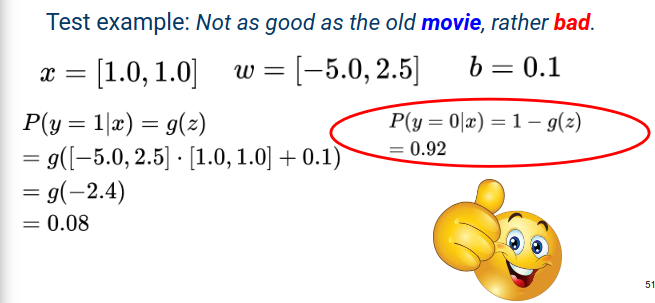
\includegraphics[trim={0.7cm 0 0 0}, clip, width=.6\linewidth]{figures/example2.png}
    \caption{Here the vector $\vec{x}$ is made up of the collection of words, here, $x_1=count(movie) \wedge x_2=count(bad)$}
\end{figure}

If we don't have the w, then we learn parameters to make the model predictions close to our labels by using a loss function (to measure the distance between the true and predicted labels) and optimization algorithm (to minimize the function usually through gradient descent.)

\begin{definition}[Logistic Regression]\label{eq:logistic-regression}
    How close is the predicted distribution Q to the true distribution P
    \begin{equation*}
        H(P,Q) = -\sum_i P(y_i)\log Q(y_i)
    \end{equation*}
\end{definition}

\subsubsection{Multiple Classes}

In the case where we have words

\begin{align*}
    x_1 (bad) & = 1 \\
    x_2 (good) & = 1 \\
    x_3 (and) & = 2 \\
\end{align*}

With sentiment analysis over 3 classes (+, -, and neutral), weights and bias are learnt per class. Then, they use a softmax function over the result of finding $z_i$.

\begin{equation*}
    y=g(z_i)=\frac{e^{z_i}}{\sum^k_{j=1}e^{z_j}}
\end{equation*}

\subsubsection{Summary}

Logistic Regression considers the importance of feautres, so is better (than Naive Bayes) at dealing with correlated feautres, also better (than Naive Bayes) with larger datasets.

\subsection{Neural Networks (NNs)}

\begin{definition}[Linear Layer]
    \begin{equation*}
        z = w \cdot x + b = \sum^I_{i=0}w_ix_i + b
    \end{equation*}
\end{definition}

\begin{definition}[Non-linear activation function]
    \begin{equation*}
        y = g(z)
    \end{equation*}
\end{definition}

\begin{definition}[Fully-connected layers]
    \begin{equation*}
        FFN(x) = (g^2(g^1(xW^1+b^1))W^2 + b^2)W^3 + b^3
    \end{equation*}
\end{definition}

The neural networks allow for automatically learning dense feature representations (or alternatively pre-trained dense representations), not one-hot encodings.

\subsubsection{Document Representation}

How to get a document representation of sentence of
fixed dimensionality?

Average of sentence - bad idea:
    
Model architecutre fixed to sentence length size, model wieghts learnt for specific word positions

\subsubsection{Neural Networks}

Automatically learned features; flexibility to fit highly complex relationships in data, but they require more data to learn more complex patterns.

\subsection{Recurrent neural networks (RNNs)}

\begin{figure}[H]
    \centering
    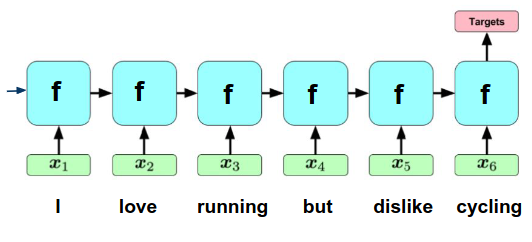
\includegraphics[width=.6\linewidth]{figures/RNN.png}    
\end{figure}

Natural language data is made up of sequences, so its natural to represent in a RNN; the value of a unit depends on own previous outputs - the last hidden state is the input to the output layer. The words are input into the model after an embedding layer which vecotrizes the ipnut.

\begin{figure}[H]
    \centering
    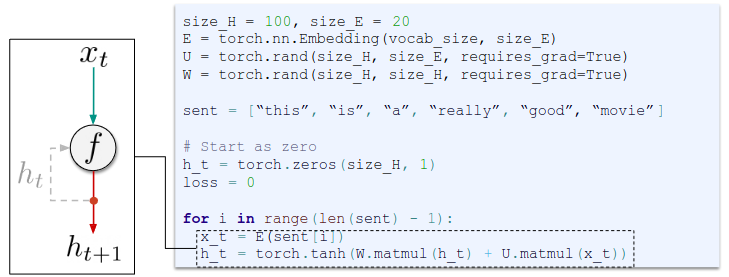
\includegraphics[width=.6\linewidth]{figures/VanillaRNN.png}    
\end{figure}

\subsubsection{Vanishing gradient problem}

The model is less able to learn from earlier inputs (Tanh derivatives are between 0 and 1) (Sigmoid derivatives are between 0 and 0.25) - Gradient for earlier layers involves repeated multiplication
of the same matrix W - depending on the dominant eignevalue this can cause gradients to either `vanish' or `explode'

\begin{warning}
    RNNs perform better when you need to understand longer range dependencies
\end{warning}

\subsection{CNNs}

CNNs are composed of a series of convolution layers,
pooling layers and fully connected layers. Convolutional layers Detect important patterns in the inputs. Pooling layers Reduce dimensionality of features and transform them into a fixed-size. Fully connected layers Train weights of learned representation for a specific task.

We can stack multiple filters on-top of eachother also.

\begin{warning}
    CNNs can perform well if the task involves key phrase recognition.
\end{warning}

\subsection{Accuracy and F1}

\begin{definition}[accuracy]
    \begin{equation*}
        Accuracy = \frac{TP + TN}{TP +FP + TN + FN}
    \end{equation*}
\end{definition}

\begin{definition}[f1-measure]
    \begin{equation*}
        f1 = 2 \times \frac{precision\times recall}{precision + recall} = \frac{TP}{TP + 0.5 (FP +FN)}
    \end{equation*}
\end{definition}

\subsubsection{Macro averaging}

averaging of each class F1 scores: increases the emphasis on less frequent classes

\subsubsection{Micro averaging}

TPs, TNs,  FNs. FPs are summed across each class.

\subsubsection{Microaveraged F1}

\begin{figure}[H]
    \centering
    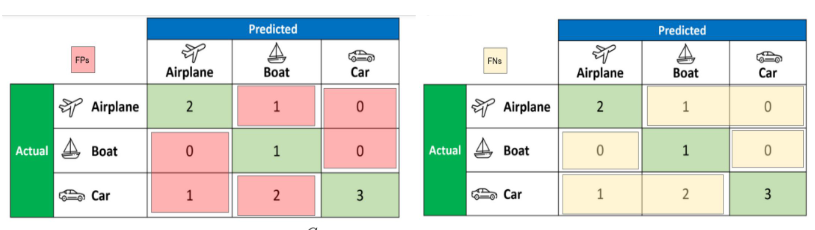
\includegraphics[trim={0 .5cm 0 0}, clip, width=.9\linewidth]{figures/f1.png}    
\end{figure}

\begin{equation*}
    \frac{\sum^C_i TP_i}{\sum^C_i TP_i + 0.5 (\sum^C_i FP_i + \sum^C_i FN_i)} = \frac{\sum^C_i TP_i}{|Dataset|} = Accuracy
\end{equation*}

\section{Language Models}

\subsection{Definition}

\begin{definition}
    Language modeling involves assigning probabilities to sequences of words. This could involve, predicting the next word in a sqeunce of words, or predicting a masked word in a sentence.

    ``Models that assign probabilities to sequences of words are called language models''\cite{book-speech-and-language-processing}
\end{definition}

\subsubsection{Uni-directional}

Here we use information from the left of the sentence to generate predictions about words that will appear to the right.

\subsubsection{Bi-directional}

Here we use information from both sides of the mask to 'fill in the gap'

\subsection{N-Gram Modelling}

The task of computing $P(w|h)$, the probability of a word w given some history h.
\begin{equation*}
    =P(w_n|w_1^{n-1})
\end{equation*}

One way to estimate this probability is from relative frequency counts: take a very large corpus, count the number of times we see the history and count the number of times that $w$ directly followed the history.

\begin{equation*}
    P(\text{the}|\text{its water is so transparent that}) = \frac{C(\text{its water is so transparent that the})}{C(\text{its water is so transparent that})}   
\end{equation*}

However, this doesn't work for long histories. This is because language is creative; new sentences are created all the time, and we won't always be able to count entire sentence. Even simple legal extensions of the example sentence may have counts of zero on the web.

\textbf{The intuition of the n-gram model is that instead of computing the probability of a word given its entire history, we can approximate the history by just the last few words.}

\begin{align*}
    P(\text{the}|\text{its water is so transparent that}) = Full\ context & = P(w_n|w_1^{n-1}) \\
    Unigram\ approximation & \approx P(w_n) = P(\text{the}) \\
    Bigram\ approximation & \approx P(w_n|w_{n-1}) = P(\text{the}|\text{that}) \\
    Triagram\ approximation & \approx P(w_n|w_{n-2,n-1}) = P(\text{the}|\text{transparent\ that})
\end{align*}

\begin{definition}[N-gram modelling]
    The N-gram models approximat ehistory by just the few last words with relation
    \begin{equation*}
        P(w_n|w_1^{n-1}) \approx P(w_n|w_{n-N+1}^{n-1})
    \end{equation*}\label{def:n-gram} 
\end{definition}

We can then estimate these probabilities as `MLE as relative frequencies' 

\begin{equation*}
    P(w_n|w_1^{n-1}) \approx P(w_n|w_{n-N+1}^{n-1}) = \frac{C(w_{n-N+1}^{n-1}w_n)}{C(w_{n-N+1}^{n-1})}
\end{equation*}

The larger, the better the counts - larger n possible, however, trigams are often enough. 

\begin{figure}[H]
    \centering
    \subfigure[shows the bigram counts from a piece of a bigram grammar from the Berkeley Restaurant Project. Note that the majority of the values are zero. In fact, we have chosen the sample words to cohere with each other; a matrix selected from a random set of eight words would be even more sparse~\cite{book-speech-and-language-processing}]{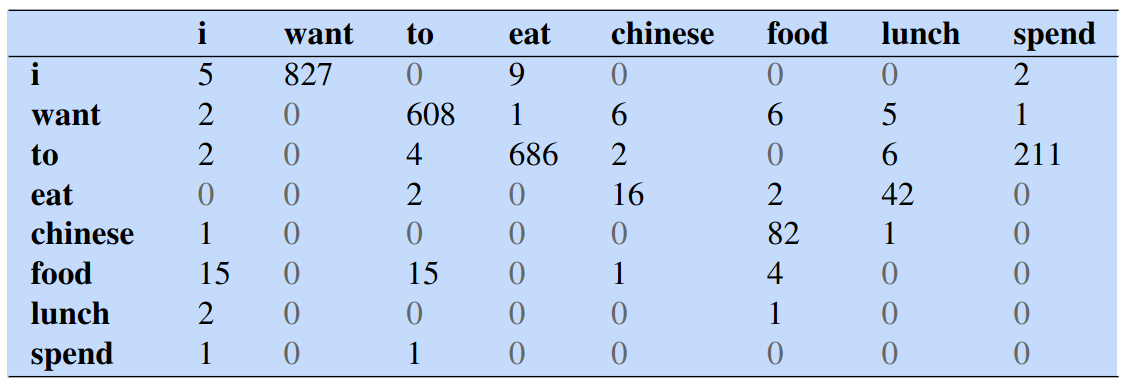
\includegraphics[width=.6\linewidth]{figures/n-gram-table-example.png}}
    \subfigure[Shows total occurrances of each word~\cite{book-speech-and-language-processing}]{
\includegraphics[width=.6\linewidth]{figures/n-gram-table-example-occurrences-.png}}
    \subfigure[Bigram probabilities for eight words in the Berkeley Restaurant Project corpus     of 9332 sentences. Zero probabilities are in gray.~\cite{book-speech-and-language-processing}]{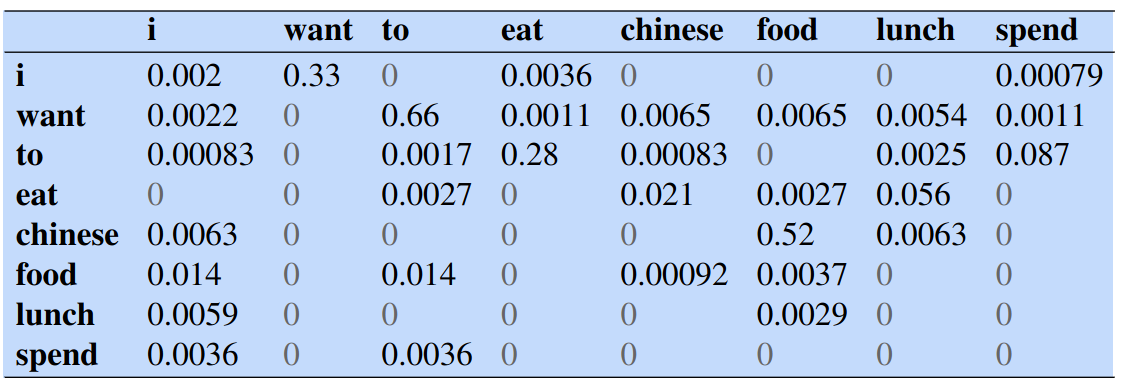
\includegraphics[width=.6\linewidth]{figures/n-gram-table-example-probs.png}}
    \caption{Bigram example}
\end{figure}

E.g. to find the probability of ``want to'' $\equiv P(to|want)$ use Definition~\ref{def:n-gram}
    
\begin{align*}
    P_{N=2}(w_n|w_1^{n-1}) & \approx P(w_n|w_{n-2+1}^{n-1}) \\
    & = \frac{C(w_{n-1}^{n-1}w_n)}{C(w_{n-1}^{n-1})} \\
    & = \frac{C(\text{to}|\text{want})}{C(\text{want})} \\
    & = \frac{C(\text{608})}{C(\text{927})} = 0.65587918
\end{align*}

\subsection{Evaluating Language Models}

We can evaluate a sequence by considering the product of conditional probabilities.

\begin{equation}\label{eq:evaluate-language-model-multiply}
    P(w_1, \ldots, w_n) = \prod^n_{k=1}P(w_k|w_1^{k-1})
\end{equation}

E.g. To find $P(<s>\text{I want chinese food}</s>)$ Given the above table and using Definition~\ref{def:n-gram}

(given also that $P(i|<s>) = 0.25 \wedge P(</s>|food) = 0.68$) 

\begin{align*}
    P_{N=2}(w_n|w_1^{n-1}) & \approx P(w_n|w_{n-2+1}^{n-1}) \\
    & = \frac{C(w_{n-1}^{n-1}w_n)}{C(w_{n-1}^{n-1})} \\
    & \Rightarrow P(i|<s>) \cdot P(want|i) \cdot P(chinese|want) \cdot P(food|chinese) \cdot P(</s>|food) \\
    & \approx 0.25 \cdot \frac{C(\text{want}|\text{i})}{C(\text{i})} \cdot \frac{C(\text{chinese}|\text{want})}{C(\text{want})} \cdot \frac{C(\text{food}|\text{chinese})}{C(\text{chinese})} \cdot 0.68 \\
    & \approx 0.25 \cdot 0.33 \cdot 0.0065 \cdot 0.52 \cdot 0.68 \\
    & = 0.000189618
\end{align*}

However, in Equation~\ref{eq:evaluate-language-model-multiply} we are multiplying many small numbers together that are less than 0. This is a very small number, so we can switch to log space \& replace multiplication by addition

\begin{align*}
    \log(P(w_1, \ldots, w_n)) = \log(\prod^n_{k=1}P(w_k|w_1^{k-1})) = \sum^n_{k=1}\log(P(w_k|w_1^{k-1}))
\end{align*}

We can then take the exponent of this.

\subsubsection{Problems with this approach}

We have an issue here with longer outputs: The longer the output is, the lower its likelihood (many multiplications give a small number)

\subsection{Perplexity}

We normalize by the length of the text `the inverse probability of a text, normalized by the \# of the words'

\begin{definition}[Perplexity]
    In practice we don't use raw probability as our metric for evaluating language models, but a variant called perplexity. The perplexity (sometimes called PPL for short) of a language model on a test set is the inverse probability of the test set, normalized by the number of words.
\end{definition}

Here $n$ is the number of words:

\begin{align*}
    PPL(w) & =P(w_1,w_2,\ldots,w_n)^\frac{-1}{N} \\
    & = \sqrt[n]{\frac{1}{P(w_1,w_2,\ldots,w_n)}}
\end{align*}
We can then use the chain rule to expand the probability of $W$
\begin{align*}
    PPL(w) & = \sqrt[n]{\frac{1}{\prod^n_{k=1}P(w_k|w_1,\ldots,w_{i-1})}} = \sqrt[n]{\frac{1}{\prod^n_{k=1}P(w_k|w_1^{k-1})}}
\end{align*}

Note that because of the inverse, the higher the conditional probability of the word sequence, the lower the perplexity. Thus, minimizing perplexity is equivalent to maximizing the test set probability according to the language model. It is a measure of the surprise in an LM when seeing new text.

\begin{itemize}
    \item if we are finding the perplexity of a single word, the best possible score is 1.
    \item if our model uniformly picks words across a vocabulary of size $|V|$, the perplexity of a single word is: $|V|$. This is becuase (as mentioned in Section~\ref{content:weighted-average-branching-factor}) if each sample has a chance $1/|V|$ of getting chosen.
\end{itemize}

\subsubsection{Summary}

Perplxeity allows us to choose the best LM for a test data: LM1 vs LM2: best LM is the one with the lowest perplexity
\begin{itemize}
    \item However, perplexity is specific to the test-set
    
    ``We can consider perplexity as the weighted average branching factor of a language. The branching factor of a language is the number of possible next words that can follow any word. Consider the task of recognizing the digits n English (zero, one, two,..., nine), given that (both in some training set and in some test set) each of the 10 digits occurs with equal probability $P=1/10$  The perplexity of this mini-language is in fact 10. To see that, imagine a test string of digits of length $N$, and assume that in the training set all the digits occurred with equal probability. \label{content:weighted-average-branching-factor}

    But suppose that the number zero is really frequent and occurs far more often than other numbers. Let’s say that 0 occur 91 times in the training set, and each of the other digits occurred 1 time each. Now we see the following test set: 0 0 0 0 0 3 0 0 0 0. We should expect the perplexity of this test set to be lower since most of the time the next number will be zero, which is very predictable, i.e. has a high probability. Thus, although the branching factor is still 10, the perplexity or weighted branching factor is smaller''~\cite{book-speech-and-language-processing}

    \item How you tokenize the data matters
\end{itemize}

\subsection{Cross Entropy Loss}

The cross-entropy is useful when we don't know the actual probability distribution p that generated some data. It allows us to use some m, which is a model of p (i.e., an approximation to p). We don't know the true distribution, e.g. the likelihood of each possible next word, we only know how many times things happen in the training data. 

Below, $q(x_i)$ is the model predicted probability of the word $x_i$ given the previous words $x_1, \ldots, x_{i-1}$:

\begin{equation*}
    H(T,q)=-\sum^N_{i=1}\frac 1 N \ln q_e(x_i)
\end{equation*}

For a single observation (from Definition~\ref{eq:logistic-regression}):

\begin{align*}
    H(P,Q) = -\sum_i P(y_i)\log Q(y_i) 
\end{align*}    

\subsubsection{Maximum Likelihood Estimation}

\begin{itemize}
    \item Consider $\mathbb{X} = {x_1, \ldots, x_n}$ examples drawn independently form a true but unknown data generating distirbution $p_{data}(x)$.
    \item Let $p_{model}(x;\theta)$ be a parametric family of probability distributions over the same space indexed by $\theta$. In other words, $p_{model}(x;\theta)$ maps any configuration x to a real number estimating the true probability $p_{data}(x)$.
    \item The maximum likelihood estimator for $\theta$ is $\arg \max _\theta p_{model}(\mathbb{X};\theta) = \arg \max _\theta \prod_{x\in \mathbb{X}} p_{model}(x;\theta)$
    \item since this is prone to numerical underflow, we go into the logarithm space: \\ $\arg \max_\theta \sum_{x\in \mathbb{X}} \log p_{model}(x;\theta)$
    \item Because the arg max does not change when we rescale the cost function, we can divide by m to obtain a version of the criterion that is expressed as an expectation with respect to the empirical distribution $\arg \max _\theta \mathbb{E}_{x\sim \hat{p}_{data}} \log p_{model}(x;\theta)$
\end{itemize}

\subsubsection{Conditional Cross-Entropy Loss}

The maximum likelihood estimator can readily be generalized to estimate a conditional probability $P(x|y;\theta)$ in order to predict y given x, we denote Y as our observed targets and X as our observed inputs. Here $\theta$ represents the parameters of the model that we're triyng to optimize.

We choose parmeters based on the loss for the whole corpus

In the given sequence of equations, the objective is transformed from maximizing the likelihood estimation to minimizing the negative log-likelihood. This is equivalent to minimizing the cross-entropy between the model's predictions and the true data distribution. The following steps are taken from \href{https://stats.stackexchange.com/questions/428937/mle-and-cross-entropy-for-conditional-probabilities/477867#477867}{this link}.

\begin{eqnarray} 
    \hat{\theta}_{ML} &=& \arg\max_{\theta} p_{model}(Y|X;\theta) \label{eq:MLE-0} \\
    &=& \arg\max_{\theta} \frac{1}{N} \prod_{i=1}^{N} p_{model}(y^{(i)}|x^{(i)};\theta) \label{eq:MLE-1} \\
    &=& \arg\max_{\theta} \frac{1}{N} \sum_{i=1}^{N} \log p_{model}(y^{(i)}|x^{(i)};\theta) \label{eq:MLE-1} \\
    &=& \arg\min_{\theta} \frac{1}{N} \sum_{i=1}^{N} - \log p_{model}(y^{(i)}|x^{(i)};\theta)  \label{eq:MLE-2} \\
    &=& \arg\min_{\theta} \frac{1}{N} \sum_{i=1}^{N} - \log p_{model}(y^{(i)}|x^{(i)};\theta) - \log p(x^{(i)}) \label{eq:MLE-3} \\
    &=& \arg\min_{\theta} \frac{1}{N} \sum_{i=1}^{N} - \log p_{model}(y^{(i)}|x^{(i)};\theta) - \log p_{model}(x^{(i)}|\theta) \label{eq:MLE-4} \\
    &=& \arg\min_{\theta} \frac{1}{N} \sum_{i=1}^{N} - \log \left( p_{model}(y^{(i)}|x^{(i)};\theta)p_{model}(x^{(i)}|\theta) \right) \label{eq:MLE-5} \\
    &=& \arg\min_{\theta} \frac{1}{N} \sum_{i=1}^{N} - \log  p_{model}(y^{(i)}, x^{(i)}|\theta) \label{eq:MLE-6} \\
    &\approx& \arg\min_{\theta} \left(\mathbb{E}_{p_{data}(x,y)}\left[ -\log p_{model}(y,x|\theta) \right] \right) \label{eq:MLE-7} \\
    &=& \arg\min_{\theta} \left(\mathbb{E}_{p_{data}(x,y)}\left[ -\log p_{model(\theta)}(y,x) \right] \right) \label{eq:MLE-8} 
\end{eqnarray}

In step~\ref{eq:MLE-3} we turn it into a minimisation problem. In step~\ref{eq:MLE-4} we subtracted logarithm of true and unknown probability of drawing the sample $x_i$, which does not change the argmax, as it is independent of $\theta$. In step~\ref{eq:MLE-5} we redefine $p_{model}(x^{(i)}|\theta) \equiv p_{model}(x^{(i)}|\theta)$ since our model is actually not modeling probability of the sample $x_i$

    % \begin{align}
    %     H(P,Q) & = -\sum_{x \in \mathcal{X}} P(x)\log q(x) \quad \text{Here $x$ refers to $(x,y)$} \\
    %     & = \arg \min_\theta \frac 1 N \sum ^N_{i=1} -\log  p_{model} (y^{(i)}|x^{(i)}; \theta) \quad \text{Sample $x,y$ from the dataset for an approximation} \\
    %     & = \arg \min_\theta \frac 1 N \sum ^N_{i=1} -\log  (p_{model} (y^{(i)}|x^{(i)}; \theta)p_{model} (x^{(i)}|\theta)) \quad \text{Separate to conditional probabilities} \\
    %     & = \arg \min_\theta \frac 1 N \sum ^N_{i=1} -\log p_{model} (y^{(i)}|x^{(i)}; \theta) - \log p_{model} (x^{(i)}|\theta) \quad \text{Separate to two log expressions} \\
    %     & = \arg \min_\theta \frac 1 N \sum ^N_{i=1} -\log p_{model} (y^{(i)}|x^{(i)}; \theta) - \log p(x^{(i)}) \quad\text{$P_{model}(x)$ doesn't depend on theta} \\
    %     & = \arg \min_\theta \frac 1 N \sum^N_{i=1} - \log p_{model} (y^{(i)}|x^{(i)}; \theta) \quad \text{We have our loss as we expected}
    % \end{align}
    
\begin{definition}[Cross-Entropy Loss]
    \begin{equation*}
        H(T,q) = - \sum^N_{i=1} \frac 1 N \ln q(x_i)    
    \end{equation*}

    Where $q(x_i)$ is the model predicted probability of the word $x_i$ given the previous words $x_1, \ldots, x_{i-1}$:
\end{definition}

\subsection{Converting Between Cross Entropy and Loss}

if you calculate Cross Entropy to the base e (if it is in base two then it is $2^H$)

\begin{equation*}
    Perplexity(M) = e^H 
\end{equation*}

\subsection{Extrinsic vs Intrinsic Evaluation}

If the goal of the languag model is to support with another task, the best choice of language model is the one that improves downstream task performance the most (extrinsic evaluation). Perplexity is less useful in this case (intrinsic evaluation).

\printbibliography
\addcontentsline{toc}{section}{Bibliography}

\end{document}